\subsection{Developers} \label{subsection:foundation-piracy-developers}
Especially for software developers, piracy is a problem.
At first glance, the problem seems to only be theft, where somebody steals a developer's \gls{ip} and redistributes it without the developer’s involvement which results in a loss of revenue.
People are then downloading an application either for free or pay the pirate and thus do not generate revenue for the originator.
\newline
At second glance, the problems are even more complex.
Income for the developer is not only lost when the user is not paying for the software, the pirate can also influence the follow up revenue by modifying the application itself.
There are two main types of revenue not generated by the purchase of the application.
The first type is the in-app purchase.
They are a popular source of income for so called freemium applications or lite versions of apps.
In case of the the freemium app, the download is for free and and includes all features. In-app purchases, e.g. in-app currency, enable the user to proceed faster or to buy cosmetic modifications.
The lite version application is a little bit different. The download is free as well but the application comes with a restricted feature set or limited time of use.
In order to take advantage of the unlocked feature set the user can buy the full license via in-app purchase.
Apps can include a mix and various degrees of theses variants.
Pirates can disable the payments for the features, enabling users to receive the in-app purchase for free and thus no earnings are generated for the developer.
\newline
The second type of follow up revenue is generated by showing in-app Ads.
When this feature is included, advertisements are shown inside the application and the developer is paid by the amount of ads seen and clicked by the user.
The Ad Unit ID \cite{googleAdmob} is responsible to assign earnings generated by an mobile advertisement to the developer.
When an application is pirated, this code can be replaced by the pirate's one. Future revenues generated by advertisements in the application will not be assigned to the developer but redirected to the pirate.
\newline
\begin{figure}[h]
    \centering
    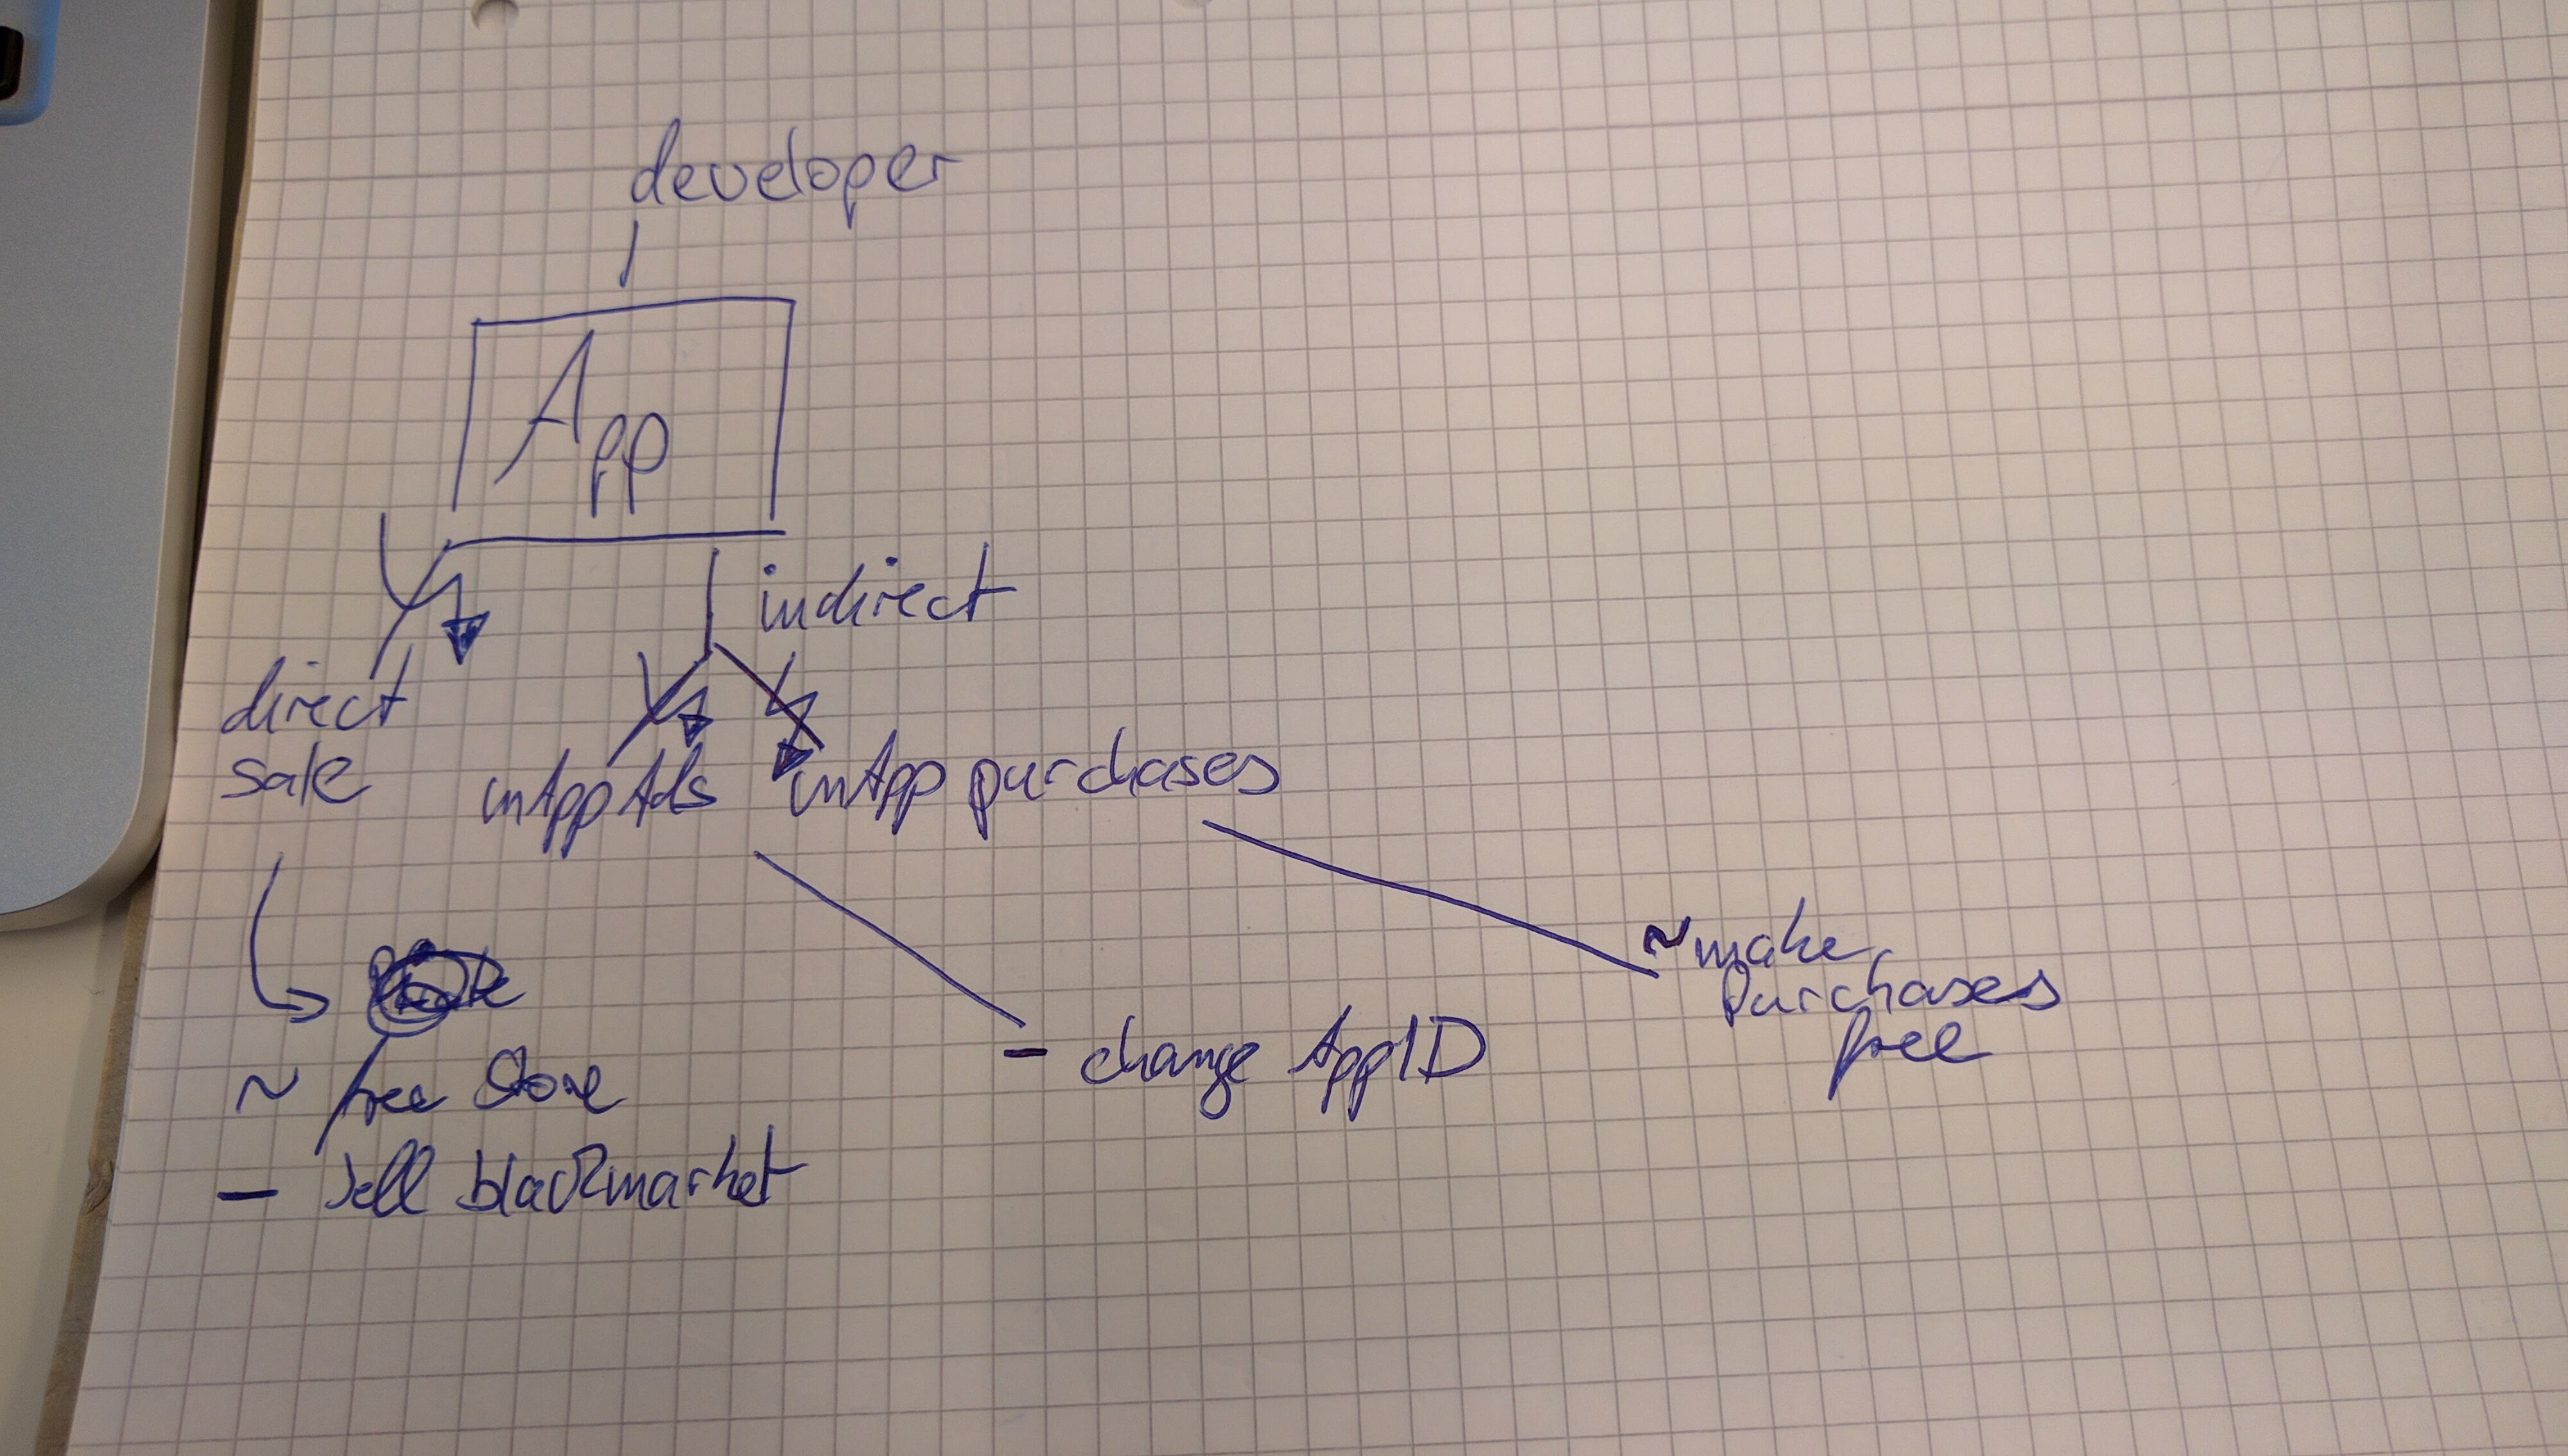
\includegraphics[width=0.8\textwidth]{data/revenue.jpg}
    \caption{Different ways to generate revenue}
    \label{fig:revenue}
\end{figure}
Beside monetary issues, additional problems arise when the app is moved to a black market store or website  and distributed without the environment of an official app store.
This results in the loss of control over the application for the developer.
It means the developer can no longer provide the users support or updates for the application to fix crashes caused by malfunctions or security issues.
Users which do not know that they are using a pirated version will connect the unsatisfying behaviour to the developer.
This can result in the loss of future revenues which are not even connected to this application.
In addition to the loss over the application this can cause unpredictable scenarios.
Since the developer cannot monitor the growth of the application over tools which are included in the marketplace of choice, he can face unpredictable high traffic.
This can stress the server because they were not scaled to the growth.
As revenue from the application is stolen, there may not be money for upgrades necessary by legal and illegal use \cite{lierschDeveloperThreats}.
\newline
\newline
Developers make a living of their applications.
When they do not earn money, because the revenue stream is redirected, because their \gls{ip} is stolen and commercialized by someone else, or if they even lose money due to uncovered maintaining costs, they cannot continue with developing and their skills are lost.
